\documentclass{llncs}

\usepackage{graphicx,epsfig,amssymb,amsmath,todonotes}
\usepackage{mathpartir}
\usepackage{xspace}
\usepackage[colorlinks=true]{hyperref}
\usepackage{algorithm,algpseudocode}
\usepackage{tikz}

\usepackage[utf8]{inputenc}
\usepackage{newunicodechar}
\newunicodechar{∃}{\ensuremath{\exists}}
\newunicodechar{∀}{\ensuremath{\forall}}
\newunicodechar{θ}{\ensuremath{\theta}}
\newunicodechar{τ}{\ensuremath{\tau}}
\newunicodechar{φ}{\ensuremath{\varphi}}
\newunicodechar{π}{\ensuremath{\pi}}
\newunicodechar{α}{\ensuremath{\alpha}}
\newunicodechar{β}{\ensuremath{\beta}}
\newunicodechar{γ}{\ensuremath{\gamma}}
\newunicodechar{δ}{\ensuremath{\delta}}
\newunicodechar{ε}{\ensuremath{\epsilon}}
\newunicodechar{λ}{\ensuremath{\lambda}}
\newunicodechar{ρ}{\ensuremath{\rho}}
\newunicodechar{σ}{\ensuremath{\sigma}}
\newunicodechar{ω}{\ensuremath{\omega}}
\newunicodechar{Γ}{\ensuremath{\Gamma}}
\newunicodechar{Φ}{\ensuremath{\Phi}}
\newunicodechar{Δ}{\ensuremath{\Delta}}
\newunicodechar{Σ}{\ensuremath{\Sigma}}
\newunicodechar{Π}{\ensuremath{\Pi}}
\newunicodechar{Θ}{\ensuremath{\Theta}}
\newunicodechar{⇒}{\ensuremath{\Rightarrow}}
\newunicodechar{⇐}{\ensuremath{\Leftarrow}}
\newunicodechar{⇔}{\ensuremath{\Leftrightarrow}}
\newunicodechar{→}{\ensuremath{\rightarrow}}
\newunicodechar{←}{\ensuremath{\leftarrow}}
\newunicodechar{↔}{\ensuremath{\leftrightarrow}}
\newunicodechar{¬}{\ensuremath{\neg}}
\newunicodechar{∧}{\ensuremath{\land}}
\newunicodechar{∨}{\ensuremath{\lor}}
\newunicodechar{≠}{\ensuremath{\neq}}
\newunicodechar{≡}{\ensuremath{\equiv}}
\newunicodechar{∼}{\ensuremath{\sim}}
\newunicodechar{≈}{\ensuremath{\approx}}
\newunicodechar{≥}{\ensuremath{\geq}}
\newunicodechar{≤}{\ensuremath{\leq}}
\newunicodechar{≫}{\ensuremath{\gg}}
\newunicodechar{≪}{\ensuremath{\ll}}
\newunicodechar{∅}{\ensuremath{\emptyset}}
\newunicodechar{⊆}{\ensuremath{\subseteq}}
\newunicodechar{⊂}{\ensuremath{\subset}}
\newunicodechar{∩}{\ensuremath{\cap}}
\newunicodechar{∪}{\ensuremath{\cup}}
\newunicodechar{∈}{\ensuremath{\in}}
\newunicodechar{⊤}{\ensuremath{\top}}
\newunicodechar{⊥}{\ensuremath{\bot}}
\newunicodechar{₀}{\ensuremath{_0}}
\newunicodechar{₁}{\ensuremath{_1}}
\newunicodechar{₂}{\ensuremath{_2}}
\newunicodechar{₃}{\ensuremath{_3}}
\newunicodechar{₄}{\ensuremath{_4}}
\newunicodechar{₅}{\ensuremath{_5}}
\newunicodechar{₆}{\ensuremath{_6}}
\newunicodechar{₇}{\ensuremath{_7}}
\newunicodechar{₈}{\ensuremath{_8}}
\newunicodechar{₉}{\ensuremath{_9}}
\newunicodechar{⁰}{\ensuremath{^0}}
\newunicodechar{¹}{\ensuremath{^1}}
\newunicodechar{²}{\ensuremath{^2}}
\newunicodechar{³}{\ensuremath{^3}}
\newunicodechar{⁴}{\ensuremath{^4}}
\newunicodechar{⁵}{\ensuremath{^5}}
\newunicodechar{⁶}{\ensuremath{^6}}
\newunicodechar{⁷}{\ensuremath{^7}}
\newunicodechar{⁸}{\ensuremath{^8}}
\newunicodechar{⁹}{\ensuremath{^9}}
\newunicodechar{ℝ}{\ensuremath{\mathbb{R}}}
\newunicodechar{ℕ}{\ensuremath{\mathbb{N}}}
\newunicodechar{ℂ}{\ensuremath{\mathbb{C}}}
\newunicodechar{ℚ}{\ensuremath{\mathbb{Q}}}
\newunicodechar{ℤ}{\ensuremath{\mathbb{Z}}}
\newunicodechar{✓}{\checkmark}
\newunicodechar{✗}{\ensuremath{\times}}
\newunicodechar{◊}{\ensuremath{\lozenge}}
\newunicodechar{□}{\ensuremath{\square}}

\newcommand{\thLemI}{\textsf{ThLemI}\xspace}
\newcommand{\thLem}{\textsf{ThLem}\xspace}
\newcommand{\spltI}{\textsf{SplitI}\xspace}
\newcommand{\splt}{\textsf{Split}\xspace}
\newcommand{\weaken}{\textsf{Weakening}\xspace}
\newcommand{\weakenI}{\textsf{WeakeningI}\xspace}

\newcommand{\dReal}{\textsf{dReal3}\xspace}
\newcommand{\zthree}{\textsf{Z3}\xspace}
\newcommand{\mathsat}{\textsf{MathSat5}\xspace}
\newcommand{\smtinterpol}{\textsf{SmtInterpol}\xspace}
\newcommand{\princess}{\textsf{Princess}\xspace}


\newcommand{\lrf}{\mathcal{L}_{\mathbb{R}_{\mathcal{F}}}}
%\newtheorem{definition}{Definition}
\newtheorem{notation}{Notation}
%\newtheorem{example}{Example}
%\newtheorem{proposition}{Proposition}
%\newtheorem{remark}{Remark}
%\newtheorem{theorem}{Theorem}

\begin{document}

% we have 15 pages + 2 pages biblio

\title{Interpolants in Nonlinear Theories over the Reals}
\author{Sicun Gao \and Damien Zufferey}
\institute{MIT}

\maketitle

\begin{abstract}
We develop algorithms for computing Craig interpolants for first-order formulas over real numbers with a wide range of nonlinear functions, including transcendental functions and differential equations.
We transform proof traces from δ-complete decision procedures into interpolants that consist of Boolean combinations of linear constraints.
The algorithms are guaranteed to find the interpolants between two formulas $A$ and $B$ whenever $A ∧ B$ is not δ-satisfiable.
At the same time, by exploiting δ-perturbations one can parameterize the algorithm to find interpolants with different positions between $A$ and $B$.
We show applications of the methods in control and robotic design, and hybrid system verification.  

\end{abstract}

\section{Introduction}
\label{sec:intro}

Difficulty. 

A concrete example of what we can compute. 

Applications. 


\section{Preliminaries}
\label{sec:prelim}

\paragraph{Craig interpolation~\cite{MR0104564}.}
We consider Craig interplants for quantifier-free first-order formulas. Given two formulas $A$ and $B$, such that $A ∧ B$ is unsatisfiable, an interpolant $I$ is a formula satisfying:
\todo{should we use ⇒ or $\entails$. I would rather keep $\entails$ for the proof trees.}
\begin{itemize}
\item $A ⇒ I$;
\item $B ∧ I ⇒ ⊥$;
\item $fv(I) ⊆ fv(A) ∩ fv(B)$ where $fv$ returns the free variables in a formula.
\end{itemize}

\paragraph{Nonlinear first-order theories over the reals.} 

We consider first-order formulas interpreted over the real numbers. Our special focus is formulas that can contain arbitrary nonlinear functions that are {\em Type 2 computable}~\cite{CAbook,vasco}. Intuitively, Type 2 computability corresponds to {\em numerical computability}. For our purpose, it is enough to note that this set of functions consist of all common elementary functions, as well as solutions of Lipschitz-continuous ordinary differential equations. Thus the first-order language is extremely expressive... \todo{why the ... ???}

\paragraph{Interval constraint propagation.}

Interval Constraint Propagation (ICP)~\cite{handbookICP} finds
solutions of real constraints using the \emph{branch-and-prune} method, combining
interval arithmetic and constraint propagation. The idea is to use interval
extensions of functions to \emph{prune} out sets of points that are not in the
solution set and \emph{branch} on intervals when
such pruning can not be done, recursively until a small enough box
that may contain a solution is found or inconsistency is observed.
A high-level description of the decision version of ICP is given in Algorithm~\ref{icpalgo}~\cite{handbookICP,DBLP:conf/cade/GaoAC12}.
The boxes, or interval domains, are written as $\vec D$ and $c_i$ denotes the $i$th constraint.
\begin{algorithm}\label{algo1}
\caption{ICP($c_1,...,c_m, \vec D = D_1\times\cdots\times D_n, \delta$)}\label{icpalgo}
\begin{algorithmic}[1]
\Statex
    \State $S \gets \vec D$
    \While{$S \neq \emptyset$}
        \State $\vec D \gets S.\mathrm{pop}()$
        \While{$\exists 1 \leq i \leq m, \vec D \neq_{\delta} \mathrm{Prune}(\vec D,c_i)$}
        \State $\vec D \gets \mathrm{Prune}(\vec D, c_i)$
        \EndWhile
        \If{$\vec D \neq \emptyset$}
            \If{$\exists 1\leq i\leq m, |\sharp c_i(\vec D)|\geq \delta$}
                \State $\{\vec D_1,\vec D_2\} \gets \mathrm{Branch}(\vec D, i)$
                \State $S.\mathrm{push}(\vec D_1)$
                \State $S.\mathrm{push}(\vec D_2)$
            \Else
                \State \Return {\sf sat}
            \EndIf
        \EndIf
    \EndWhile
    \State \Return {\sf unsat}
\end{algorithmic}
\end{algorithm}





\paragraph{Proofs from constraint propagation.}

The complete theory behind proof extraction from $\delta$-decision procedure is available in~\cite{DBLP:conf/synasc/GaoKC14}.
Here, we described a simplified version.
The proof is divides the solution space until it can prove, using interval arithmetic, that each small piece of the solution space is empty.
The solver uses constraints propagation and pruning steps to limit the amount of branching required.
However, the proof it produces only need to consider two main rules: splitting and theory lemma.
The rules are shown in Figure~\ref{fig:rules}. \todo{caption of that fig}
The \splt rules divides the solution space into two disjoint subspaces.
The theory lemmas (\thLem) are the leaves of the proof.
They occurs when the solver managed to prove the absence of solution in a given subspace.
The interval constraints propagation algorithms works on one constraint at the time. 
The \weaken rule extracts those conjunct out of the main formula.

Each step of the proof has a set of variables $\vec x$ with a domain $\vec D$ and $F$ is a formula.
We use of vectors in the formulas, writing $\vec x ∈ \vec D$ to denote $\bigwedge_i x_i ∈ D_i$.
The domains are intervals, i.e., each $D_i$ has the form $[l_i,u_i]$ where $l_i$,$u_i$ are the lower and upper bounds for $x_i$.
Since we are looking at unsatisfiability proofs, each node implies $⊥$.

The root of the proof is has formula $A ∧ B$ and $D$ covers the entire domain,
the inner nodes are \splt.
and the proof's leaves are theory lemmas directly followed by a weakening.

\begin{notation}
Conjunction binds stronger. Intervals assume well-definedness. 
\end{notation}

\begin{figure}
\centering
\begin{mathpar}
\inferrule{ {} }{
  \vec x ∈ \vec D ∧ c \entails ⊥
}{(\thLem)}\\

\inferrule{
  C := c ∧ \bigwedge_k C_k \\
  \vec x ∈ \vec D ∧ c \entails ⊥
}{
  \vec x ∈ \vec D ∧ C \entails ⊥
}{(\weaken)}\\

\inferrule{
  x_i ∈ [l_i, p] ∧ \bigwedge_{j ≠ i} x_j ∈ D_j ∧ C \entails ⊥ \\\\
  x_i ∈ [p, u_i] ∧ \bigwedge_{j ≠ i} x_j ∈ D_j ∧ C \entails ⊥
}{
  x_i\in [l_i, u_i] \wedge \bigwedge_{j\neq i} x_j∈ D_j ∧ C \entails ⊥
}{(\splt)}
\end{mathpar}
\caption{Proof rules for ICP}
\label{fig:rules}
\end{figure}

Algorithm~\ref{icpalgo} generates proof during the \emph{branching} and \emph{pruning} operations.
Branching directly corresponds to the $\splt$ rule.
Pruning, on the other hand, is a combination of the three rules.
Let us look at $\vec D' = \text{Pruning}(\vec D, c_i)$.
The constraint $c_i$ is selected with the \weaken.
For each $D'_i=[l',u']$ which is strictly smaller than $D_i=[l,u]$, the \splt and \thLem rules are applied.
If $l'>l$ then we split on $l$ and a lemma shows that the interval $[l',l]$ has no solution.
The same is done for the upper bounds $u'$,$u$.
Figure~\ref{fig:prune} shows a pruning step and the corresponding proof.

\begin{figure}
\centering
\begin{tikzpicture}
\node (n0) at (-1.2, 0.1) {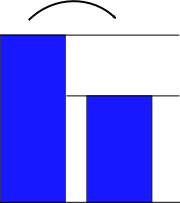
\includegraphics[scale=0.4]{img/pruning.pdf}};
\node (n1) at ( 0.0, 0.85) {$u$};
\node (n2) at ( 0.05, 0.2) {$u'$};
\node (n3) at ( 0.0,-1.0) {$l$};
\node (n4) at (-1.0, 1.5) {pruning by $c_i$};
\node (n5) at (0.8, -0.2) {\large \ldots};
\node (n6) at (6.0, 0.0) {\begin{minipage}{0.7\textwidth}
{\small
\begin{mathpar}
\inferrule{
    \vdots\\
    \inferrule{
        \inferrule{ {} }{ x ∈ [u',u] ∧ c_i \entails ⊥ }{(\thLem)}
    }{
        x ∈ [u',u] ∧ c_i ∧ \bigwedge_{k≠i} c_k \entails ⊥ 
    }{(\weaken)} \\
}{
    x ∈ [l,u] ∧ \bigwedge_k c_k \entails ⊥
}{(\splt)}
\end{mathpar}
}
\end{minipage}
};
\end{tikzpicture}
\caption{Pruning operation and the corresponding proof}
\label{fig:prune}
\end{figure}

\section{Interpolants in Nonlinear Theories}
\label{sec:itp}

Introduce various parameters/templates for the interpolants. 
\begin{itemize}
	\item Robustness
	\item Boolean operations
	\item Degrees 
\end{itemize}


\subsection{Disjunctive Linear Interpolants}

Algorithms for the generation from proof trees to disjunctions of linear constraints. 

Let $l$ be a labelling function that maps formula and variables to \textsc{a},\textsc{b}, or \textsc{ab}.
For each proof rule we associate an partial interpolant, written in square bracket on the right of the conclusion of the rules.

% need a labelling function
% ThLem: A → false 
%        B → true
% Split: A → I₁ ∨ I₂
%       AB → ite(x_i ≤ p, I₁, I₂) 
%        B → I₁ ∧ I₂
% Weakening: identify

\begin{mathpar}
\inferrule{ {} }{
  \vec x ∈ \vec D ∧ c \entails ⊥ \quad [l(f) ≠ \textsc{a}]
}{(\thLemI)}\\

\inferrule{
  C = c ∧ \bigwedge_k C_k \\
  \vec x ∈ \vec D ∧ c \entails ⊥ \quad [I]
}{
  \vec x ∈ \vec D ∧ C \entails ⊥ \quad [I]
}{(\weakenI)}\\


\inferrule{
  x_i ∈ [l_i, p] ∧ \bigwedge_{j ≠ i} x_j ∈ D_j ∧ C \entails ⊥ \quad [I₁] \\\\
  x_i ∈ [p, u_i] ∧ \bigwedge_{j ≠ i} x_j ∈ D_j ∧ C \entails ⊥ \quad [I₂] 
}{
  x_i\in [l_i, u_i]\wedge \bigwedge_{j\neq i} x_j ∈ \vec D_j ∧ C \entails ⊥ \quad
  \left[ \substack{ I₁ ∨ I₂     \qquad \quad ~~  \text{if} ~ l(x_i) = \textsc{a} \\
                    ite(x_i < p, I₁, I₂) ~~ \text{if} ~ l(x_i) = \textsc{ab}\\
                    I₁ ∧ I₂     \qquad \quad ~~  \text{if} ~ l(x_i) = \textsc{b}}\right]
}{(\spltI)}

\end{mathpar}

where $ite(x,y,z)$ is a shorthand for $(x ∧ y)∨(¬x ∧ z)$

\todo[inline]{find a better way to format that.}

Intuitively, a proof of unsatisfiability is a tiling of the solution space where each tile is associated with a conjunct $f$ from $A ∧ B$.
$f$ is a witness that shows the absence of solution in a given tile.
The interpolation rules traverse the rules and selects which tiles belong to the interpolant $I$.

At the leaf level (rule \thLemI), the tile is in $I$ if $f$ is not part of $A$, i.e., the contradiction originates from $B$.
If $f$ is in both $A$ and $B$ then it can be considered as either part of $A$ or $B$.
Both cases leads to a correct interpolant.
The \weakenI rule does not influence the interpolant, it is only required to pick $f$ from $A ∧ B$.

The \spltI is the most interesting rule.
Splitting the domains essentially defined the bounds of the subsequent tiles.
Let $x$ be the variable whose domain is split at value $p$ and $I₁$, $I₂$ be the two interpolants for the case when $x < p$ and $x ≥ p$.
If $x$ occurs in $A$ but not $B$, then $x$ cannot occur in $I$.
Since $x$ is in $A$ then we know that $A$ implies $x < p ⇒ I₁$ and $x ≥ p ⇒ I₂$.
Eliminating $x$ give $I = I₁ ∨ I₂$.
A similar reasoning is applicable when $x$ occurs in $B$ but not $A$ and gives $I = I₁ ∧ I₂$.
When $x$ occurs in both $A$ and $B$ then $x$ is kept in $I$ and acts as a selector for the values of $x$ smaller than $p$ $I₁$ is selected, otherwise $I₂$ applies.

The correctness of our method is shown by the following theorem:
\begin{theorem}
The rules \spltI, \thLemI, \weakenI generate a Craig interpolant $I$ from the proof of unsatisfiability of $A$ and $B$.
\label{thm:sound}
\end{theorem}
\begin{proof}
%\emph{(Sketch)}
We prove correctness of the rules by induction.
To express the inductive invariant, we split the domain $\vec D$ into the domains $\vec D_A$ and $\vec D_B$ which contains only the intervals of the variables occuring in $A$, $B$ respectively.

At any given point in the proof, at any given point in the proof the partial interpolant $I$ is an interpolant for the formula $A$ over $\vec D_A$ and $B$ over $\vec D_B$.
At the root of the proof tree we get an interpolant for the whole domain $\vec D = \vec D_A ∧ \vec D_B$.

At the leaves of the proof, or the \thLemI rule, one of the constrain has no solution over the domain.
Let's assume that this constraint comes from $A$.
Then the partial interpolant $I$ is $⊥$.
We have that $A ∧ \vec D_A ⇒ I$ by the semantics of the \thLem rule ($⊥⇒⊥$).
Trivially $B ∧ \vec D_B ∧ I ⇒ ⊥$ and $fv(I) = ∅ ⊆ fv(A) ∩ fv(B)$.
When the contradiction comes from $B$, a similar reasoning is applied with $I=⊤$.

The \weakenI only serves to select which constraint cause the contradiction and does not changed the invariant.

The \spltI rule is the most complex case.
We have to consider whether the variable $x$ which is split come from $A$, $B$, or is shared.
For instance, if $x\in fv(A)$ then the induction step has $\vec D_{A1} = \vec D_A ∧ x < p$ and $\vec D_{A2} = \vec D_A ∧ x ≥ p$ and $\vec D_B$ is unchanged.
if $x ∈ fv(B)$ then $\vec D_B$ is affected and $\vec D_A$ is unchanged.
if $x$ is shared then both $\vec D_A$ and $\vec D_B$ are affected.

Let consider that $x ∈ fv(A)$ and $x ∉ fv(B)$.
We omit the case where $x$ is in $B$ but not $A$ as it is similar.
The induction hypothesis is\\
\parbox{0.35\linewidth}{
\begin{eqnarray*}
& A ∧ (\vec D_A ∧ x < p) ⇒ I₁ \\
& A ∧ (\vec D_A ∧ x ≥ p) ⇒ I₂ \\
& B ∧ \vec D_B ∧ I₁ ⇒ ⊥ \\
& B ∧ \vec D_B ∧ I₂ ⇒ ⊥
\end{eqnarray*}
}
which simplifies to
\parbox{0.35\linewidth}{
\begin{eqnarray*}
& A ∧ \vec D_A ⇒ I₁ ∨ I₂ \\
& B ∧ \vec D_B ∧ (I₁ ∨ I₂) ⇒ ⊥
\end{eqnarray*}
}.

Finally, we need to consider $x ∈ fv(A)$ and $x ∈ fv(B)$.
The induction hypothesis is\\
\parbox{0.38\linewidth}{
\begin{eqnarray*}
& A ∧ (\vec D_A ∧ x < p) ⇒ I₁ \\
& A ∧ (\vec D_A ∧ x ≥ p) ⇒ I₂ \\
& B ∧ (\vec D_B ∧ x < p) ∧ I₁ ⇒ ⊥ \\
& B ∧ (\vec D_B ∧ x ≥ p) ∧ I₂ ⇒ ⊥
\end{eqnarray*}
}
which simplifies to
\parbox{0.42\linewidth}{
\begin{eqnarray*}
& A ∧ \vec D_A ⇒ ite(x < p, I₁, I₂)\\
& B ∧ \vec D_B ∧ ite(x < p, I₁, I₂) ⇒ ⊥
\end{eqnarray*}
}.
\qed
\end{proof}

\begin{example}
If we look at proof for the example in Figure~\ref{fig:example}, we get the following proof and interpolant

\todo[inline]{this is partial version that still need formatting...}

\begin{mathpar}
\inferrule{
    \inferrule{
        \inferrule{
            \vdots
        }{
            x \in [-1,1] \land y \in [0,0.26] \land A \land B \entails \bot [ I' ]
        }{(\spltI)}
        \inferrule{
            \inferrule{
                {}
            }{
                x \in [-1,1] \land y \in [0.26,1] \land B \entails \bot [ \top ]
            }{(\thLemI)}
        }{
            x \in [-1,1] \land y \in [0.26,1] \land A \land B \entails \bot [ \top ]
        }{(\weakenI)}
    }{
        x \in [-1,1] \land y \in [0,1] \land A \land B \entails \bot [ 0.26 \leq y \lor (y \leq 0.26 \land I') ]
    }{(\spltI)}
    \inferrule{
        \inferrule{
            {}
        }{
            x \in [-1,1] \land y \in [-1,0] \land A \entails \bot [ \bot ]
        }{(\thLemI)}
    }{
        x \in [-1,1] \land y \in [-1,0] \land A \land B \entails \bot [ \bot ]
    }{(\weakenI)}
}{
    x \in [-1,1] \land y \in [-1,1] \land A \land B \entails \bot [ 0 \leq y \land 0.26 \leq y \lor (y \leq 0.26 \land I') ]
}{(\spltI)}
\end{mathpar}
\end{example}

\subsection{Extensions}

\todo[inline]{yada ...}

\paragraph{δ-interpolants.}
The interpolation method that we propose uses a δ-decision procedure to build a Craig interpolant.
The properties of the interpolant means that $A ∧ ¬I$ and $B ∧ I$ are both unsatisfiable.
However, they are not necessarily δ-unsatisfiable.

To obtain an interpolant such that both $A ∧ ¬I$ and $B ∧ I$ are δ-unsatisfiable, we can weaken both $A$ and $B$ by a factor δ.
However, $A$ and $B$ must be at least $3δ$-unsatisfiable to guarantee that the solver finds a proof of unsatisfiability.
Furthermore, we can also introduce perturbation only on one side in other to make the interpolant stronger of weaker.

\paragraph{Boolean structure.}
In the previous section, we shown how to compute an interpolant for the conjunctive fragment of quantififer-free nonlinear theories over ℝ.
However, in many cases formula also contains disjunctions.
To handle disjunctions, our method can be combined with the method presented by Yorsh and Musuvathi~\cite{DBLP:conf/cade/YorshM05} for building an interpolant from a resolution proof where some of the proof's leaves are interpolant for specific theory.


\paragraph{Interpolant strength.}
Do to the similarity of our method to interpolation of propositional formula we can borrow result about adapting the interpolant strenght from D'Silva et.al.~\cite{DBLP:conf/vmcai/DSilvaKPW10} to our framework.
\todo[inline]{give some details}

\section{Examples and Experiments}
\label{sec:eval}

We have implemented the interpolation algorithm in a modified version of the \dReal which is available at \url{https://github.com/dzufferey/dreal3/}.
The interpolation hooks at the places where the proof is produced.
Since the proofs produced by \dReal can be very large,i.e., gigabytes, the interpolants are built and simplified on-the-fly.
The full proof is not kept.


\section{Related Work and Future Work}
\label{sec:related}


\section{Conclusion and Future Work}
\label{sec:concl}

We present an method for computing Craig interpolants for first-order formulas over real numbers with a wide range of nonlinear functions.
Our method transform proof traces from δ decision procedures into interpolants consisting of disjunctive linear constraints.
The algorithms are guaranteed to find the interpolants between two formulas $A$ and $B$ whenever $A ∧ B$ is not δ-satisfiable.
Furthermore, we show how the framework apply to systems of ordinary differential equations.
We implemented our interpolation algorithm in the \dReal SMT-solver and apply the method to domains such robotic design, and hybrid system verification.  

In the future, we plan to expand our work to richer proof systems.
The ICP loop produces proof based on interval pruning which results in large, ``squarish'' interpolants.
Using more general proof systems, e.g. cutting planes, we will be able to get smaller, smoother interpolants.
CDCL-style reasoning for richer theories, e.g., LA(ℝ)~\cite{DBLP:conf/cav/McMillanKS09} and polynomial~\cite{DBLP:conf/cade/JovanovicM12}, is a likely basis for such extensions.
Furthermore, we are interested in investigating the link between classical interpolation and Craig interpolation over the reals.
Using methods like spline interpolation and radial basis functions, it maybe possible to build smoother interpolants.
%We also to extend the our rules to compute interpolants mixed proofs with both integer and real variables.


\bibliographystyle{abbrv}
\bibliography{biblio,refs}

\appendix
%\begin{proof}
We prove correctness of the interpolation rules by induction.
\paragraph{Base case: \textsc{ThLemI} rule}
if $l(f)=A$ and $I=⊥$ then
\begin{itemize}
\item $A ⇒ I$: if $l(f)=A$ the theroy lemma means that $A⇔⊥$, thus, $⊥⇒⊥$
\item $B ∧ I ⇒ ⊥$: trivially $⊥⇒⊥$
\item $fv(I) ⊆ fv(A) ∩ fv(B)$: trivial
\end{itemize}

else we have $l(f)=B$ and $I=\top$, so
\begin{itemize}
\item $A ⇒ I$: trivially $\top ⇒ \top$
\item $B ∧ I ⇒ ⊥$:  if $l(f)=B$ the theroy lemma means that $A⇔⊥$, thus, $⊥⇒⊥$
\item $fv(I) ⊆ fv(A) ∩ fv(B)$: trivial
\end{itemize}

\paragraph{Induction step 1: \textsc{WeakeningI} rule}
\begin{itemize}
\item $A ⇒ I$: by induction hypothesis
\item $B ∧ I ⇒ ⊥$: by induction hypothesis
\item $fv(I) ⊆ fv(A) ∩ fv(B)$: by induction hypothesis
\end{itemize}

\paragraph{Induction step 2: \textsc{SplitI} rule}
The trick is how to apply the induction hypothesis.
We have to consider 3 cases:
\begin{enumerate}
\item $x ∈ fv(A) ∧ x \notin fv(B)$ and $I = I₁ ∨ I₂$
\item $x ∈ fv(A) ∧ x ∈ fv(B)$ and $I = ite(x < p, I₁, I₂)$
\item $x \notin fv(A) ∧ x ∈ fv(B)$ and $I = I₁ ∧ I₂$
\end{enumerate}

Let's divide the domain $D$ into $D_A$ and $D_B$ where each contains the range of the corresponding variables.
Variables that are in both side have their domain in both $D_A$ and $D_B$. 
if $x\in fv(A)$ then the induction step has $D_{A1} = D_A ∧ x < p$ and $D_{A2} = D_A ∧ x ≥ p$ and $D_B$ is unchanged.

In the first case, the induction hypothesis is
\begin{eqnarray*}
& A ∧ x_i < p ⇒ I₁ \\
& A ∧ x_i ≥ p ⇒ I₂ \\
& B ∧ I₁ ⇒ ⊥ \\
& B ∧ I₂ ⇒ ⊥
\end{eqnarray*}
which simplifies to:
\begin{eqnarray*}
& A ⇒ I₁ ∨ I₂ \\
& B ∧ (I₁ ∨ I₂) ⇒ ⊥
\end{eqnarray*}

In the second case, the induction hypothesis is
\begin{eqnarray*}
& A ∧ x_i < p ⇒ I₁ \\
& A ∧ x_i ≥ p ⇒ I₂ \\
& B ∧ x_i < p ∧ I₁ ⇒ ⊥ \\
& B ∧ x_i ≥ p ∧ I₂ ⇒ ⊥
\end{eqnarray*}

The first two equations gives
\[
    ¬ A ∨ (¬(x < p) ∨ I₁) ∧ (¬(x ≥ p) ∨ I₂)
\]
which is the same as $¬ A ∨ ite(x < p, I₁, I₂)$
and, therefore, $A ⇒ ite(x < p, I₁, I₂)$.

The last two equations gives
\[
    ¬ B ∨ ((¬(x < p) ∨ ¬ I₁) ∧ (¬(x ≥ p) ∨ ¬ I₂))
\]
using distributivity law we get
\[
    ¬ B ∨ (x ≥ p ∧ ¬ I₂) ∨ (x < p ∧ ¬ I₁) ∨ (¬ I₁ ∧ ¬ I₂)
\]
because $(¬ I₁ ∧ ¬ I₂) ⇒  (x ≥ p ∧ ¬ I₂) ∨ (x < p ∧ ¬ I₁)$
this simplifies to
\[
 ¬ B ∨ (x ≥ p ∧ ¬ I₂) ∨ (x < p ∧ ¬ I₁)
\]
which is the same as: $¬ B ∨ ¬ ite(x < p, I₁, I₂)$
and, therefore, $B ∧ ite(x < p, I₁, I₂) ⇒ ⊥$.

In the third case: the induction hypothesis is
\begin{eqnarray*}
& A ⇒ I₁ \\
& A ⇒ I₂ \\
& B ∧ x_i < p ∧ I₁ ⇒ ⊥ \\
& B ∧ x_i ≥ p ∧ I₂ ⇒ ⊥
\end{eqnarray*}
which simplifies to:
\begin{eqnarray*}
& A ⇒ I₁ ∧ I₂ \\
& B ∧ (I₁ ∧ I₂) ⇒ ⊥
\end{eqnarray*}
\end{proof}



\end{document}

